\documentclass[preprint,11pt]{elsarticle}
\usepackage{geometry}               
\geometry{letterpaper}                  
\usepackage{graphicx}
\usepackage{amssymb,amsmath}
\usepackage{epsfig,subfigure,epstopdf}
\usepackage{algorithm}
\usepackage{algorithmic}
\usepackage{rotating}

% -- David Package --
\usepackage[normalem]{ulem}
\usepackage[usenames,dvipsnames]{color}
\newcommand{\rd}{\textcolor{Red}}
\newcommand{\gr}{\textcolor{Green}}
\newcommand{\og}{\textcolor{Orange}}
\newcommand{\pp}{\textcolor{Purple}}
\usepackage[edtable]{lineno}
% -- End of package --

\newtheorem{theorem}{Theorem}[section]
\newtheorem{lemma}[theorem]{Lemma}
\newtheorem{proposition}[theorem]{Proposition}
\newtheorem{corollary}[theorem]{Corollary}
\newenvironment{proof}[1][Proof]{\begin{trivlist}
\item[\hskip \labelsep {\bfseries #1}]}{\end{trivlist}}
\newenvironment{definition}[1][Definition]{\begin{trivlist}
\item[\hskip \labelsep {\bfseries #1}]}{\end{trivlist}}
\newenvironment{example}[1][Example]{\begin{trivlist}
\item[\hskip \labelsep {\bfseries #1}]}{\end{trivlist}}
\newenvironment{remark}[1][Remark]{\begin{trivlist}
\item[\hskip \labelsep {\bfseries #1}]}{\end{trivlist}}

\DeclareGraphicsRule{.tif}{png}{.png}{`convert #1 `dirname #1`/`basename #1 .tif`.png}

\begin{document}
\begin{frontmatter}
  \title{General Linear Algebra Computing Environment}
  \author[a01]{Chenhan D. Yu} \ead{chenhan@cs.utexas.com}
  \author[a01]{Jianyu Huang} \ead{jianyu@cs.utexas.com}
  \address[a01]{Department of Computer Science, University of Texas at Austin}

  \begin{abstract}
  GLACE is a runtime system freeing user from writing multiple parallel APIs, 
  learning parallel algorithms, yet at the same time still fully exploit the computing power 
  of heterogeneous systems.
   
  After the Moore law broke, architectures of modern computers become much more 
  complex than before. The performance of sequential code is no longer portable and 
  scalable on new architectures, and the burden again goes back to programmers. 
  Recently, in order to deploy all computing resources, programmers may need to learn 
  OpenMp or Pthread for shared memory systems, MPI or socket programming for 
  distributed systems, CUDA, OpenCL or OpenGL if the system is equipped with 
  accelerators.
  
  Of course, learning these languages doesn't solve the problem. Even if programmers can 
  write these languages, they are still far away from getting high performance, since these 
  languages are just virtual programming models that facilitate programming, yet the actual 
  behaviors mapping to the hardware are hidden. An automatic parallelizing environment is 
  needed to avoid these inefficient developing processes.
  
  So our goal is to provide programmers with such an automatic parallelizing environment 
  in the domain of linear algebra. By dependency analysis, we are able to transform this 
  problem into a scheduling problem which will be solved by some new heuristic algorithms 
  later. The dependency analysis is implemented on domain languages level (a.k.a task 
  level) but not instruction level to take the advantage of some existing high performance 
  libraries such as BLAS, LAPACK.
  
  Note that the just in time (JIT) analysis frees users from any control flow, loop or function 
  call issue in parallel computing, but still cheap enough, since tasks are much fewer than 
  instructions. We compare the similarity between the existing static instruction scheduling 
  strategies and our dynamic strategies, contrasting the difference to show the limitation of 
  static analysis. At the end we will also show how this environment and the just in time 
  analysis is useful by both dense and sparse matrix computation.
  \end{abstract}
  \begin{keyword}
    Automatic parallelism \sep Task scheduling \sep
    heterogenous computing \sep graphic processing unit (GPU) \sep Intel Xeon Phi
  \end{keyword}
\end{frontmatter}

\linenumbers \linenumberdisplaymath

% ====================================================================
\section{Introduction}
% ====================================================================
  After the Moore law broke, architectures of modern computers become much more 
  complex than before, and the performance of sequential code is no longer portable and 
  scalable on new architectures. The burden again shifts from system designers back to 
  programmers, since automatic parallelization in the compiler level is still a difficult problem to 
  solve. Thus, most of the programmers choose to control multiple threads or processes 
  themselves in order to exploit the computing resources.  
  
  Recently, in order to deploy all computing resources, programmers may need to learn 
  OpenMp \cite{} or Pthread \cite{} for shared memory systems, MPI \cite{} or socket 
  programming for distributed systems, CUDA \cite{}, OpenCL \cite{} or OpenGL \cite{} if the 
  system is equipped with accelerators. 
  All the APIs above require programmers to control threads or processes explicitly, and
  OpenMP is the only API with compiler support automatic parallelization that allow user to 
  use annotations to specify the parallel section. Unfortunately, this kind of parallel model (BSP)
  has a critical problem in synchronization for unbalance loading and also is not suitable for
  heterogenous system.   
  
  
% ====================================================================
\section{Dependency Analysis}
% ====================================================================

GLACE allows users to write their program in a sequential fashion and performs run-time
  dependency analysis to exploit parallelism. Top level routines will be partitioned into smaller
  tasks that can have 3 different kinds of dependency: write after read (WAR), read after
  write (RAW), write after write (WAW). Two tasks with one of these dependencies can't 
  be executed concurrently otherwise may lead to incorrect results. 
  In GLACE, the analysis phase will be performed after the task generating by 
  using Algorithm ~\ref{alg:dep}. The algorithm is a simplified version of the dependency 
  analysis in \cite{}.     


  %Especially for the submatrix part...

  dependecy analysis


  Ernie Chan


  \subsection{Category of dependency for Matrix operations}
  \begin{enumerate}
	\item True(Flow) dependency\\
  Flow dependencies occur where a block is read by one task after it is written by a previous task (read after write).\\
  e.g.\\
  S1: A := B + C;\\
  S2: D := A + E;\\


\item Anti-dependency\\
  Anti-dependencies creates the scenarios when one task write a block after another task read the same task (write after read).\\
  e.g.\\



\item Output dependency\\
  Output dependencies take place where the output block of one operation is overwritten by subsequent computation (write after write).\\


  To simplify the dependence analysis, one of our assumption is that the operations must first read the result of one operation before overwritting it. Therefore, we only need to concentrate on flow and anti-dependencies, where output dependencies are shown as flow dependencies.[Ernie's paper]\\

  \end{enumerate}


  focus

  flow dependency notation


  The figure is too ugly. I think we may need to add the subscript to the symbol so that it looks a little "acceptable".



  Difference with Ernie Chan's work.

  \subsection{Constructing a DAG}

  In Alg[], we present the alogirhm for dynamically detecting data dependencies and constructing a DAG for dependencies relations between tasks.\\


 


% ====================================================================
\section{Data Distribution and Software Cache}
% ====================================================================
  In order to increase the data reuse rate and reduce the overhead of communication, GLACE
  implements a software cache to manage the device memory, allowing automatic data reuse. 
  Instead of the traditional cache lookup table, we use IMP model \cite{} to describe the distribution 
  of an object's locations. This enable GLACE to analysis data affinity between tasks easily and 
  also reduce the overhead of cache table looking up. In the following paragraph, we will first 
  introduce concept of distribution, and then explain how to implement the software cache with
  the distribution.    
  
  An object's distribution D(obj) represents the data locality in the distributed memory that maps 
  an object into a subset of $2^{nd+1}$, and the invertible function $F_{i,j}$ that transforms 
  distribution written in the form $D_j = F_{i, j}(D_i)$ representing 
  the required communication for redistributing $D_i$ into $D_j$. Since $F_{i, j}$ is invertible,
  $F_{i, j}^{-1} = F_{j, i}$ which is useful while the output distribution is given.  
  
  In GLACE, the host memory is the main memory and we can treat device memories as a 
  layer of cache hierarchy. Every devices can directly communication with the host memory 
  yet the communication between devices is indirect. For example, $D_1(obj) = \{d_1\}$ and 
  we would like the new distribution to include $d_2$. It is impossible for the new distribution
  to be $D_2(obj) = \{d_1, d_2\}$, since the only way to have a replica on $d_2$ is to 
  first copy the object back to the host memory, and then again copy the memory to $d_2$.
  In this case, $\{h, d_1, d_2\} = D_3(obj) = F_{1, 3}(D_1(obj))$ is the cheapest transformation
  among all possible transformations to achieve our goal, since the data movement involved 
  inside the transformation is the minima communication for the requirement.
  We will discuss the corresponding device cache actions in the next paragraph and will discuss 
  what kind of transformations is desired in the next section. 
  
  The corresponding cache actions such as fetching, writing back and replacing to these 
  distribution transformation are all happening in the fetching step before the execution if 
  there is no prefetching. Algorithm~(\ref{alg:fetch}) describes the fetching step that includes the
  distribution transformations of all arguments of a task. For each argument, if the the device
  isn't in the distribution, the device will try to fetch the memory from the host memory.
  If the host memory also isn't in the distribution, the object needs to first be written back to
  the host memory and then the device can perform fetching. 
   
  In this section, we introduce the concept of distributed distribution of an object and the 
  transformation function corresponding to the communication. 
   
    
% ====================================================================
\section{Heterogenous Performance Model}
% ====================================================================
  GLACE try to solve the optima heterogenous schedule problem by assuming that there is 
  a performance model for each task on each architecture. The performance model includes
  computation cost and communication cost. By using this model, GLACE is able to balance
  the workload on each worker and also reduces the communication amount.  

% ====== < Notation Table > ======
\begin{table}
  \centering
  {\footnotesize 
  \begin{tabular}{lllll}
    \hline
    Notation    &\ & Meaning of the notation \\  \cline{1-1}  \cline{3-3}
    {\tt nw}        && number of workers \\
    {\tt nd}         && number of devices \\
    {\tt nt}          && number of tasks \\
    \hline
    {\tt $h$}       && host memory \\
    {\tt $d_i$}    && $i$th device memory \\
    {\tt $obj$}    && distributed object \\
    \hline
    $D(obj)$      && object's distribution \\
    $F(D)$        && distribution transformation function \\
    \hline
    $CM$          && communication cost \\
    $CP$           && computation cost \\
    \hline
  \end{tabular}
}
\caption{Notations used in the hybrid CPU-GPU multifrontal methods.
  The variable $s$ and $u$ stand for the dimension of the matrix corresponding 
  to {\tt sn$_i$} and {\tt up$_i$}.}
  \label{tab:notation}
\end{table}
% ------  

% ====================================================================
\section{Scheduler}
% ====================================================================
  GLACE scheduler is responsible for dispatching ready tasks to workers' ready queue. 




 



% ====================================================================
\section{Evaluation}
% ====================================================================

We have implemented the $gemm$, $trsm$, $syrk$ routine in BLAS 3.\\

% ====== < Routine Table > ======
\begin{table}
  \centering
  {\footnotesize 
  \begin{tabular}{l|l|l|l|l}
    \hline
	Routine Name    & Abbrev. & Operation & Cost & Comment\\
	\hline
	\underline{GE}neral \underline{M}atrix-\underline{M}atrix multiplication & GEMM & $C:=\alpha AB+\beta C$ & $2mnk$ & $C \in \mathbb{R}^{m \times n}$, $A \in \mathbb{R}^{m \times k}$, $B \in \mathbb{R}^{k \times n}$  \\
	\hline
    \underline{SY}mmetric \underline{R}ank-\underline{K} & SYRK &  $C:=\alpha AA^{T}+\beta C$ & $n^2k$ & $A \in \mathbb{R}^{n \times k}$, $C \in \mathbb{R}^{n \times n}$ is symmetric, stored in lower triangular part\\
    \hline
	\underline{TR}iangular \underline{S}olve with \underline{M}ultiple right-hand sides & TRSM &  $B:=BA^{-T}$ & $mn^2$ & $B \in \mathbb{R}^{m \times n}$, $A \in \mathbb{R}^{n \times n}$ is lower triangular\\
	\hline
  \end{tabular}
}
\caption{Routine name}
  \label{tab:notation}
\end{table}
% ------  





% ====================================================================
\section{Scheduler}
% ====================================================================
  GLACE scheduler is responsible for dispatching ready tasks to workers' ready queue. 





Evaluation part







% ====================================================================
\section{Related Work}
% ====================================================================


\subsection{SuperMatrix}
In Ernie Chan’s dissertation (SuperMatrix), he has already addressed some issues we put forward in our “Goals” part. Ernie presents an application of dependence analysis and runtime data flow scheduling to matrix computations. By investigating the scheduling of matrix computations expressed as directed acyclic graphs for shared-memory parallism, Ernie provides a flexible framework for scheduling matrix computations and developed a scheduling algorithm that leverages both load balance and data locality.\\
However, as far as we see, there are still much further work we can do, as the followings,
\begin{itemize}
	\item \emph{Flexible granularity for block size}\\
		The block size for SuperMatrix is fixed, which is not flexible. We would like to make the block size adjustable in the run-time, which is a "JIT" feature.
	\item \emph{high utilization for heterogeneous architecture}\\
		Once using GPU, SuperMatrix cannot utilize CPU. We would like to exploit both CPU and GPU, i.e. construct a performance model to leverage the heterogeneous architecture to achieve high utilization.
	\item \emph{ubiquitous interface for diverse libraries}\\
		SuperMatrix is bounded with libflame library. We would like to provide ubiquitous interface for diverse libraries, instead of being restricted to libflame.
	\item \emph{broad support for multiple operations}\\
		SuperMatrix only supports dense linear algebra. We will try to support other operations such as sparse matrix computations.
\
\end{itemize}

\subsection{Instruction Scheduling}




% ====================================================================
\section{References}
% ====================================================================

	%%biblatex
	%%\renewcommand{\refname}{\CHead{d}}

\cite{lin2010application}
\cite{guyer2004broadway}
\cite{van2009libflame}
\cite{vanlibflame}
\cite{van2008science}



	\renewcommand\refname{\vskip -1cm}
	\bibliographystyle{amsplain}
	\bibliography{glace_report}








1. Ernie Chan's paper




\begin{figure}
  \centering
  \includegraphics[width=6.0in]{output1.eps} 
  \caption{1-by-1 partition}
  \label{fig:dep1}
\end{figure}
\begin{figure}
  \centering
  \includegraphics[width=6.0in]{output.eps} 
  \caption{2-by-2 partition}
  \label{fig:dep2}
\end{figure}

\begin{figure}
\begin{minipage} [t] {0.5\textwidth}
  \includegraphics[width=3.2in]{timeline1.eps} 
  \caption{Execution timeline without prefetching, green(communication), red(computation)}
  \label{fig:timeline1}
\end{minipage}
\begin{minipage} [t] {0.5\textwidth}
  \includegraphics[width=3.2in]{timeline2.eps} 
  \caption{Execution timeline without prefetching, green(communication), red(computation)}
  \label{fig:timeline2}
\end{minipage}
\end{figure}

\begin{algorithm}
\caption{{\bf (estimate).} GLACE cost estimation algorithm}
\label{alg:estimate}
{\footnotesize
\begin{algorithmic} [1]
\STATE C = estimate(worker, task)
\STATE Input: worker, task
\STATE Output: C
\STATE $CM = 0$, $CP = 0$
\IF {worker.device}
  \STATE $CP = model(worker.device, task, arguments)$
  \FOR {each argument of the task}
    \IF {worker.device $\notin$ distribution}
      \STATE $CM \pm bandwidth(sizeof(argument))$
      \IF {host $\notin$ distribution}
        \STATE $CM \pm bandwidth(sizeof(argument))$
      \ENDIF
    \ENDIF
  \ENDFOR 
\ELSE
  \STATE $CP = model(host, task, arguments)$
  \FOR {each argument of the task}
    \IF {host $\notin$ distribution}
      \STATE $CM \pm bandwidth(sizeof(argument))$
    \ENDIF
  \ENDFOR 
\ENDIF
\STATE $C = CM + CP$
\end{algorithmic}
}
\end{algorithm}

\begin{algorithm}
\caption{{\bf (fetch).} GLACE fetch algorithm}
\label{alg:fetch}
{\footnotesize
\begin{algorithmic} [1]
\STATE fetch(worker, task)
\STATE Input: worker, task
\FOR {each argument of the task}
  \STATE acquire the distribution lock   
  \IF {worker.device $\notin$ distribution}
    \IF {host $\notin$ distribution}
      \STATE pick a source from the distribution and $cache\_writeback()$
      \STATE distribution $=$ distribution $\cup$ host
    \ENDIF
    \IF {worker.device}
      \STATE $cache\_fetch()$
      \STATE distribution $=$ distribution $\cup$ worker.device
    \ENDIF
  \ENDIF
  \STATE acquire the lock of device cache
  \STATE release the distribution lock
\ENDFOR
\end{algorithmic}
}
\end{algorithm}

\begin{algorithm}
\caption{{\bf (prefetch).} GLACE prefetch algorithm}
\label{alg:prefetch}
{\footnotesize
\begin{minipage} [t] {0.4\textwidth}
\begin{algorithmic} [1]
\STATE $d2h = prefetch\_d2h(worker)$
\STATE Input: worker
\STATE Output: d2h
\IF {! isempty(worker.writeback)}
  \STATE object = head(worker.writeback)
  \IF {host $\notin$ distribution}
    \STATE $cache\_async\_writeback()$
    \STATE return TRUE
  \ENDIF
\ENDIF
\STATE return FALSE
\end{algorithmic}
\end{minipage}
\begin{minipage} [t] {0.6\textwidth}
\begin{algorithmic} [1]
\STATE $h2d = prefetch\_d2h(worker)$
\STATE Input: worker
\STATE Output: h2d 
\IF {! isempty(worker.readyqueue)}
  \STATE task $=$ head(worker.readyqueue)
  \FOR {each argument of the task}
    \IF {worker.device $\notin$ distribution}
      \IF {host $\in$ distribution}
        \STATE $cache\_async\_fetch()$
        \STATE acquire the distribution lock
        \STATE distribution $=$ distribution $\cup$ worker.device
        \STATE release the distribution lock
      \ENDIF
    \ENDIF
  \ENDFOR
\ENDIF
\end{algorithmic}
\end{minipage}
}
\end{algorithm}

\begin{algorithm}
\caption{{\bf (execute).} GLACE execute algorithm}
\label{alg:execute}
{\footnotesize
\begin{algorithmic} [1]
\STATE $execute(worker, task)$
\STATE Input: worker, task
\STATE $fetch(worker, task)$ \label{ln:simple1}
\STATE d2h $=$ $prefetch\_d2h(worker)$
\STATE h2d $=$ $prefetch\_h2d(worker)$
\STATE $kernel(arguments)$ \label{ln:simple2}
\FOR {each W or RW type argument of the task}
  \STATE distribution $=$ worker.device
  \STATE $push\_tail(worker.writeback)$  
\ENDFOR
\STATE $wait\_prefetch(worker, d2h, h2d)$
\end{algorithmic}
}
\end{algorithm}

\begin{algorithm}
\caption{{\bf (update).} GLACE dependencies update algorithm}
\label{alg:update}
{\footnotesize
\begin{algorithmic} [1]
\STATE $update(task)$
\STATE Input: task
\STATE
\end{algorithmic}
}
\end{algorithm}


\begin{algorithm}
\caption{{\bf (update).} GLACE dependencies analysis algorithm}
\label{alg:update}
{\footnotesize
\begin{algorithmic} [1]
\STATE $update(task)$
\STATE Input: Linear algebra algorithm S, block size b
\STATE Output: Directed acyclic graph $(V, E)$
\STATE $V :=  \emptyset$; $E := \emptyset$;

\FOR {each matrix A $\in \mathbb{R}^{m \times n}$}
  \FOR {$i$ from $0$ to $m/b$}
    \FOR {$j$ from $0$ to $n/b$}
      \STATE $A_{ij} \texttt{->} rset = \emptyset$; $A_{ij} \texttt{->} wset = \emptyset$;
    \ENDFOR
  \ENDFOR
\ENDFOR

%$A_{ij}$ represents the $i$th in row, $j$th in column submatrix???? blocks
\FOR {each \textbf{task} in S}
  \STATE {Store \textbf{task} into the Vertex Set: $V: = V \cup \{task\}$}

  \FOR {each $A_{ij}$ read / rw by \textbf{task}}
    \STATE { $A_{ij}\texttt{->}rset :=  A_{ij}\texttt{->}rset \cup \{task\}$}
    \IF {($A_{ij}\texttt{->}wset != \emptyset$) }
      \FOR {each element $task'$ in $A_{ij}\texttt{->}wset$}
	    \IF {$task != task'$}
	      \STATE {Add edge $E:= E \cup \{task' \rightarrow task\}$}
	    \ENDIF
      \ENDFOR
    \ENDIF
  \ENDFOR

  \FOR {each $A_{ij}$ write / rw by \textbf{task}}
    \IF {$A(i,j)\texttt{->}rset != \emptyset$}
      \FOR {each element $task'$ in $A_{ij}\texttt{->}rset$}
	    \IF {$task != task'$}
          \STATE {Add edge $E:= E \cup \{task' \rightarrow task\}$}
	    \ENDIF
       \ENDFOR
    \ENDIF 
    \STATE { $A_{ij}\texttt{->}wset :=  A_{ij}\texttt{->}wset \cup \{task\}$}
  \ENDFOR

\ENDFOR
%Submatrix -> 


\end{algorithmic}
}
\end{algorithm}




\begin{algorithm}
\caption{{\bf (worker).} GLACE worker algorithm}
\label{alg:worker}
{\footnotesize
\begin{algorithmic} [1]
\STATE $worker(worker)$
\STATE Input: worker
\WHILE {! isempty(worker.readyqueue)}
  \STATE acquire the readyqueue lock
  \STATE task $=$ $pop\_head(worker.readyqueue)$
  \STATE release the readyqueue lock
  \IF {task}
    \STATE commit $=$ $execute(worker, task)$;
    \IF {commit}
      \STATE update dependencies
    \ENDIF
  \ENDIF
\ENDWHILE
\end{algorithmic}
}
\end{algorithm}

%----------------------------------------------------------------------------------------

\end{document}
